
\chapter{Elasticity and its application}

\section{The elasticity of demand}

To measure how much demand responds to changes in its determinants, economists use the concept of \keyword{elasticity}.

\subsection{The price elasticity of demand and its determinants}

The \keyword{price elasticity of demand} measures how much the quantity demanded responds to a change in price.
Demand for a good is said to be \keyword{elastic} if the quantity demanded responds substantially to changes in the price.
Demand is said to be \keyword{inelastic} if the quantity demanded responds only slightly to changes in the price.


\subsubsection{Necessities versus luxuries}

Necessities tend to have inelastic demands, whereas luxuries have elastic demands.


\subsubsection{Availability of close substitutes}

Goods with close substitutes tend to have more elastic demand because it is easier for consumers to switch from that good to others.

\subsubsection{Definition of the market}

The elasticity of demand in any market depends on how we draw the boundaries of the market.
Narrowly defined markets tend to have more elastic demand than broadly defined markets,
because it is easier to find close substitutes for narrowly defined goods. 

\subsubsection{Time horizon}

Goods tend to have more elastic demand over longer time horizons.


\subsection{Computing the price elasticity of demand}

\begin{equation}
  \text{Price elasticity of demand} = \frac{\text{Percentage change in quantity demanded}}{\text{Percentage change in price}}
\end{equation}

\subsection{The midpoint method}

If you try calculating the price elasticity of demand between two points on a demand curve, you will quickly notice an annoying problem: The elasticity from point A to point B seems different from the elasticity from point B to point A.
One way to avoid this problem is to use the \keyword{midpoint method} for calculating elasticities.



We can express the midpoint method with the following formula for the price elasticity of demand between two points,
denoted $(Q_1, P_1)$ and $(Q_2, P_2)$:
\begin{equation}
  \text{Price elasticity of demand} = \frac{(Q_2-Q_1)/[(Q_2+Q_1)/2]}{(P_2-P_1)/[(P_2+P_1)/2]}
\end{equation}


\subsection{The variety of demand curves}

Economists classify demand curves according to their elasticity.
Demand is \keyword{elastic} when the elasticity is greater than 1, so that quantity moves proportionately more than the price.
Demand is \keyword{inelastic} when the elasticity is less than 1, so that quantity moves proportionately less than the price.
If the elasticity is exactly 1, so that quantity moves the same amount proportionately as price, demand is said to have \keyword{unit elasticity}.


\subsection{Total revenue and the price elasticity of demand}

\begin{tcolorbox}
  \keyword{total revenue}
  the amount paid by buyers and received by sellers of a good,
  computerd as the price of the good $P$ times the quantity sold $Q$
  \begin{equation}
    \text{total renenue} = P\times Q
  \end{equation}

  As show in Figure \ref{fig:total-revenue}.
\end{tcolorbox}

\begin{figure}[!ht]
  \centering
  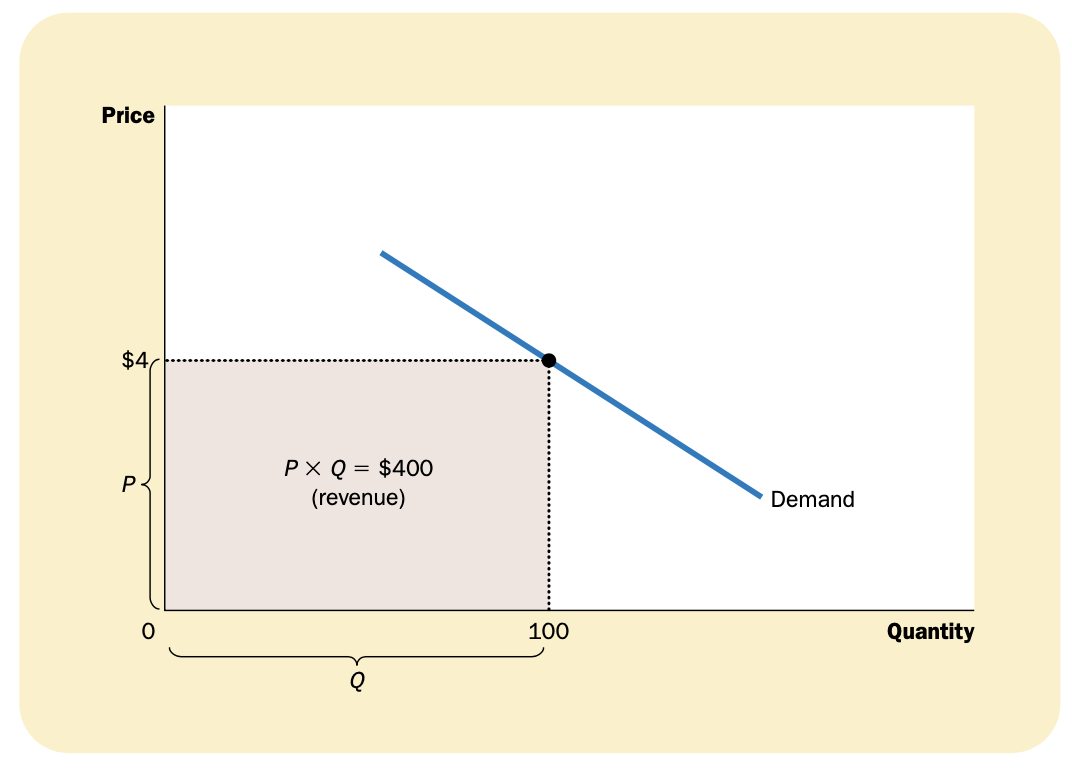
\includegraphics[width=\textwidth]{pics/total-revenue}
  \caption{Total revenue}
  \label{fig:total-revenue}
\end{figure}

\begin{tcolorbox}
  General rule:
  \begin{itemize}
  \item When a demand curve is inelastic (a price elasticity less than 1), a price increase raises total revenue, and a price decrease reduces total revenue.
  \item When a demand curve is elastic (a price elasticity greater than 1), a price increase reduces total revenue, and a price decrease raises total revenue.
  \item In the special case of unit elastic demand (a price elasticity exactly equal to 1), a change in the price does not affect total revenue.
  \end{itemize}

  As shown in Figure \ref{fig:inelastic-demand} and \ref{fig:elastic-demand}.
\end{tcolorbox}


\begin{figure}[!ht]
  \centering
  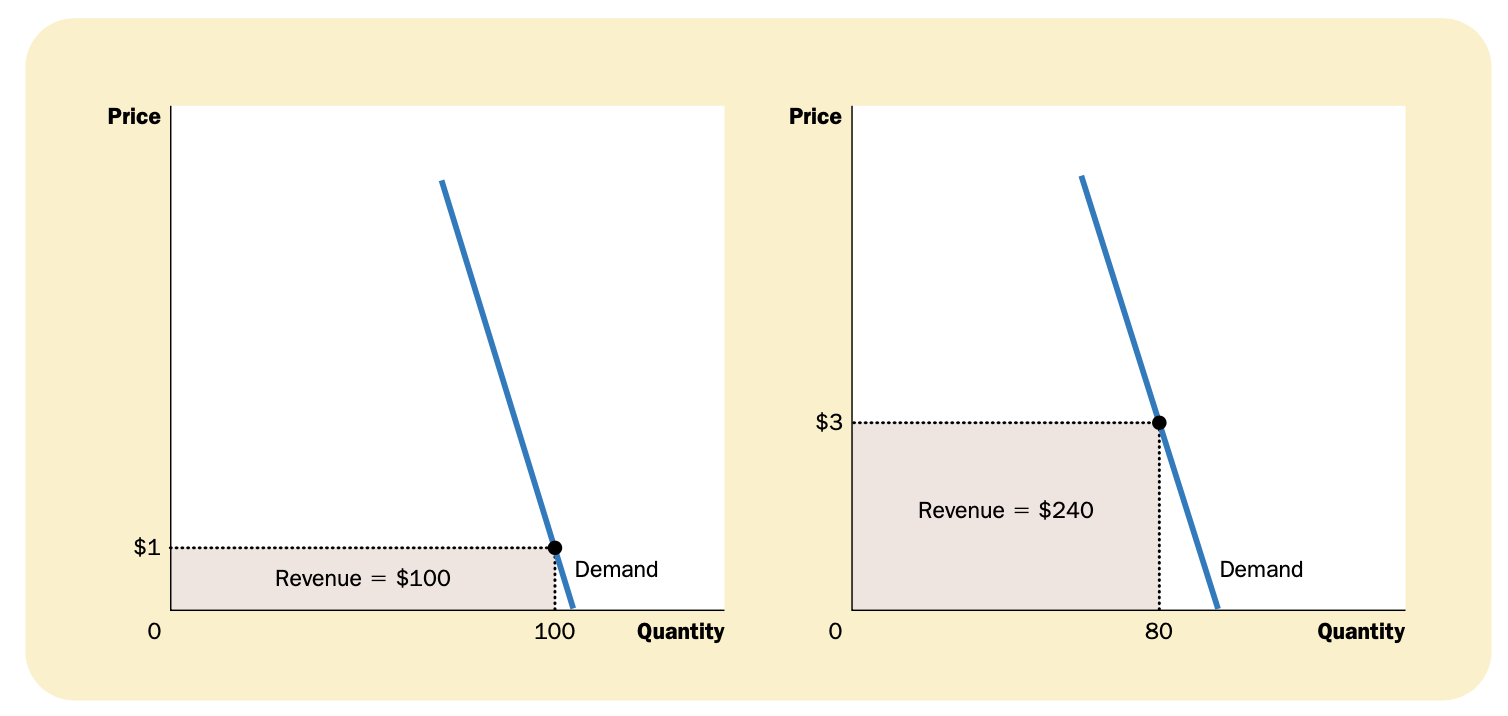
\includegraphics[width=\textwidth]{pics/inelastic-demand}
  \caption{Inelastic demand}
  \label{fig:inelastic-demand}
\end{figure}

\begin{figure}[!ht]
  \centering
  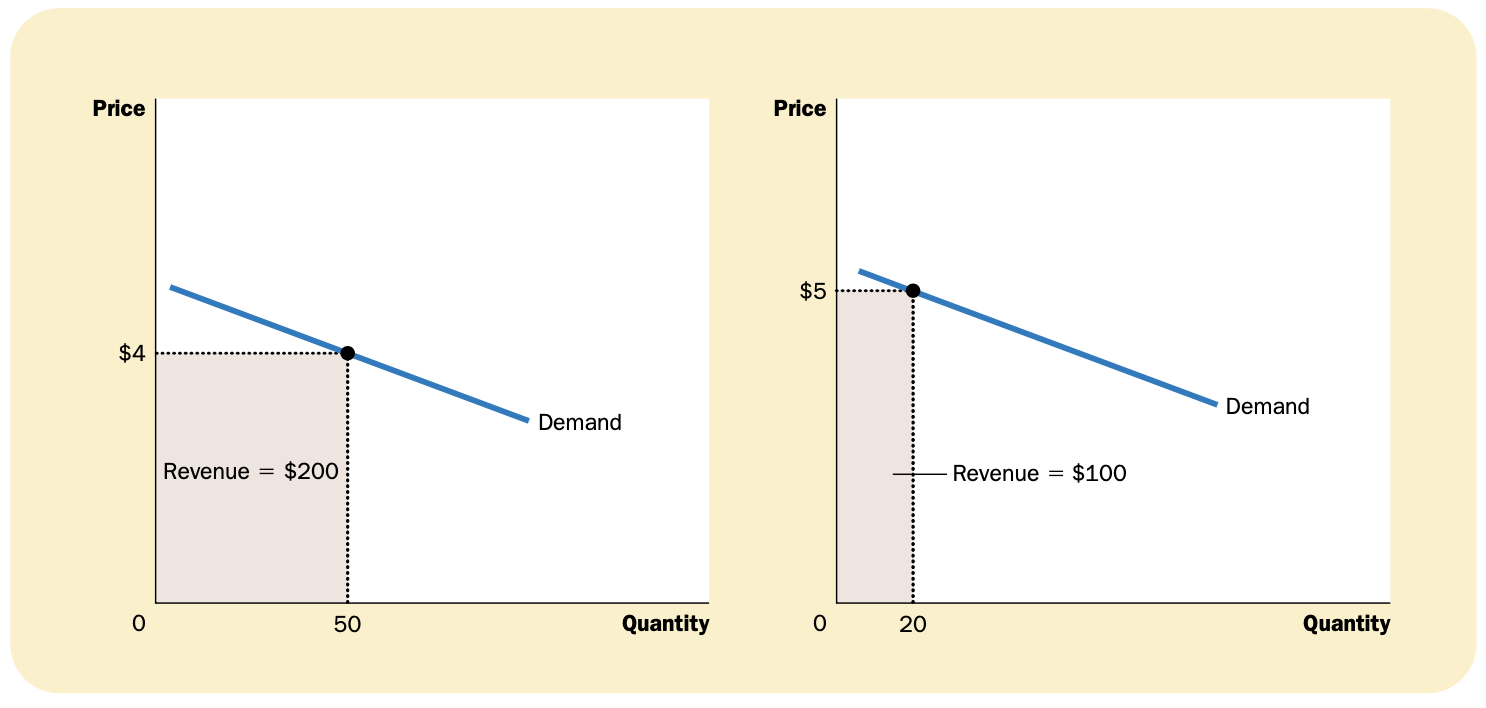
\includegraphics[width=\textwidth]{pics/elastic-demand}
  \caption{Elastic demand}
  \label{fig:elastic-demand}
\end{figure}

\subsection{Other demand eslasticities}

\subsubsection{The income elasticity of demand}

Economists use the \keyword{income elasticity of demand} to measure how the quantity demanded changes as consumer income changes.

\begin{equation}
  \text{Income elasticity of demand} = \frac{\text{Percentage change in quantity demanded}}{\text{Percentage change in income}}
\end{equation}

\subsubsection{The cross-price elasticity of demand}

Economists use the \keyword{cross-price elasticity of demand} to measure how the quantity demanded of one good changes as the price of another good changes.

\begin{equation}
  \text{Cross-price elasticity of demand} = \frac{\text{Percentage change in quantity demanded of good 1}}{\text{Percentage change in the price of good 2}}
\end{equation}


\section{The elasticity of supply}

\subsection{The price elasticity of supply and its determinants}

The \keyword{price elasticity of supply} measures how much the quantity supplied responds to changes in the price.

\subsection{Computing the price elasticity of supply}

\begin{equation}
  \text{Price elasticity of supply} = \frac{\text{Percentage change in quantity supplied}}{\text{Percentage change in price}}
\end{equation}


